\begin{frame}
  \frametitle{Transient Calculations}
  % a comment
  Load Following Results:
  \begin{figure}[htbp!]
        \begin{center}
        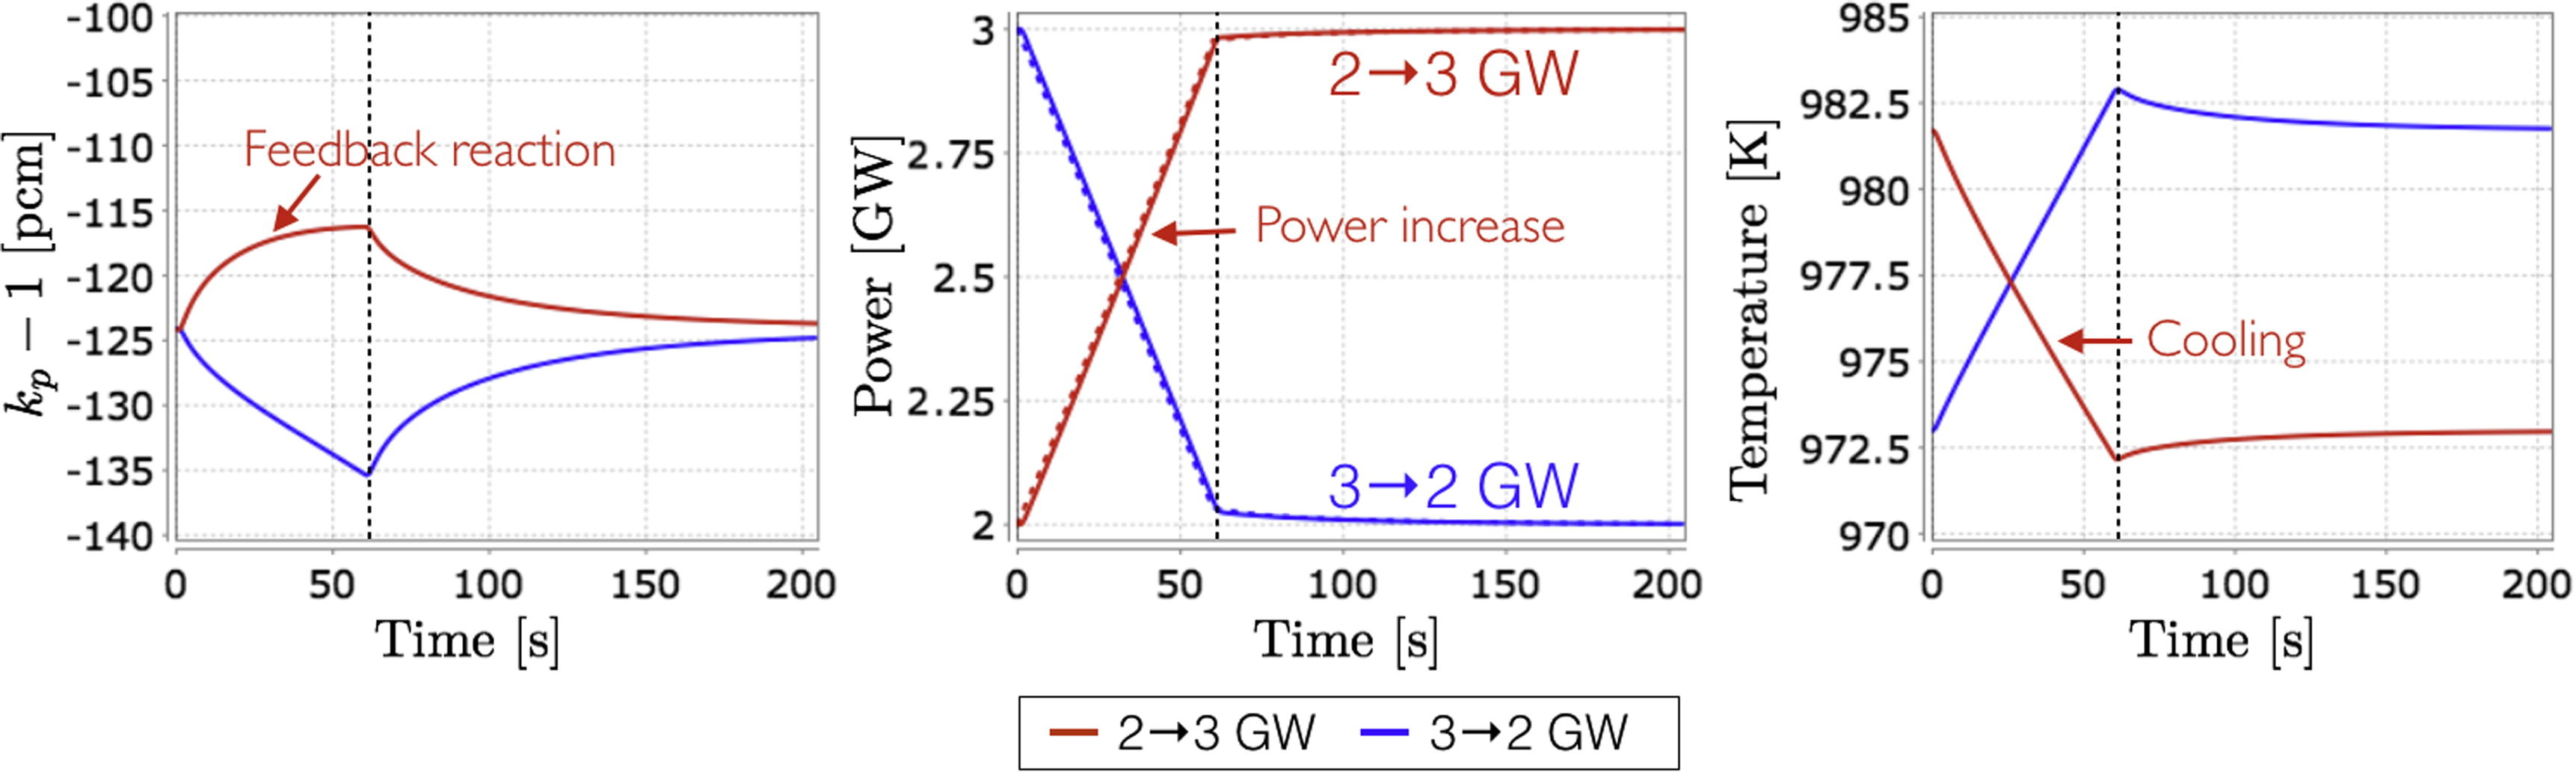
\includegraphics[scale=0.65]{JC-Oct16/transient-effects.jpg}
        \end{center}
        \caption{Evolution of metrics for 33\% power variation in 60 s.}
        \label{fig:transient}
  \end{figure}
        No active regulation of reactivity, don't need control rods to 


\end{frame}

\begin{frame}
\frametitle{Transient Calculations (cont.)}
        Overcooling Accident Results:
        \begin{figure}[htbp!]
                \begin{center}
                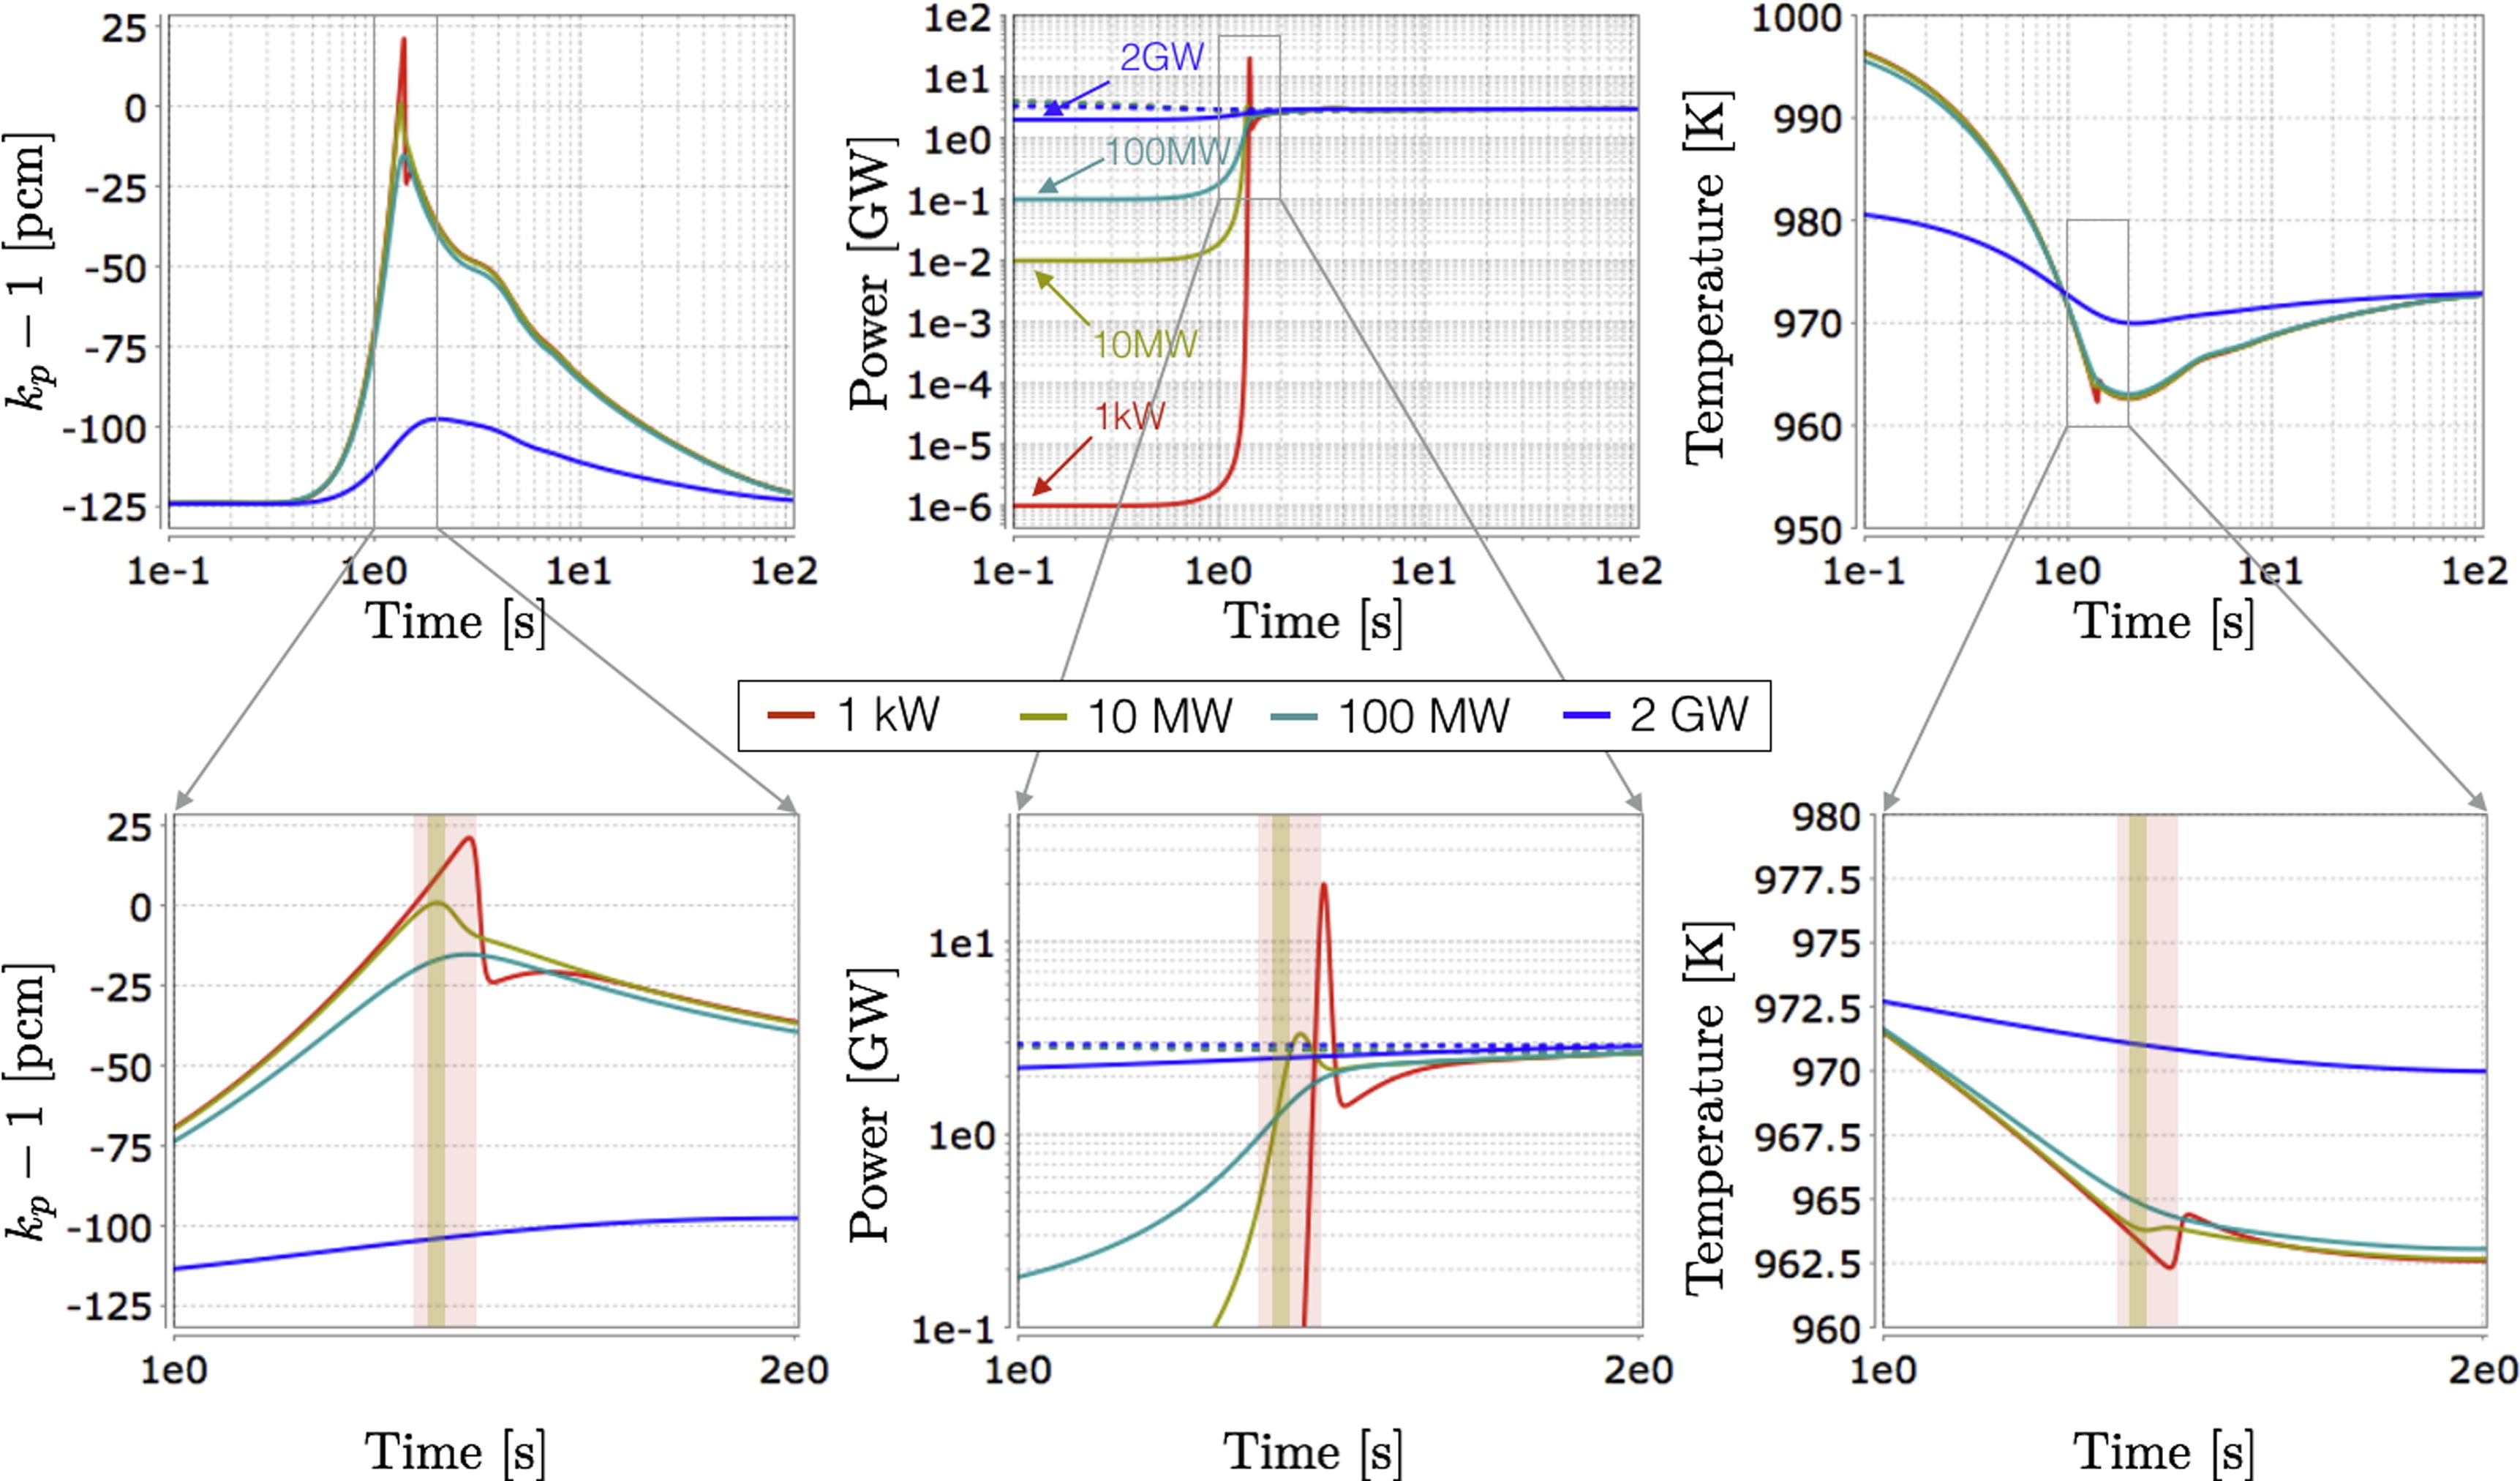
\includegraphics[scale=0.5]{JC-Oct16/overcooling-effects.jpg}
                \end{center}
                \caption{Evolution of metrics for instantaneous overcooling.}
                \label{fig:overcooling}
        \end{figure}


\end{frame}

\begin{frame}
        \frametitle{Transient Calculations (cont.)}
                Overcooling Accident Results (cont.):
                \begin{figure}[htbp!]
                        \begin{center}
                        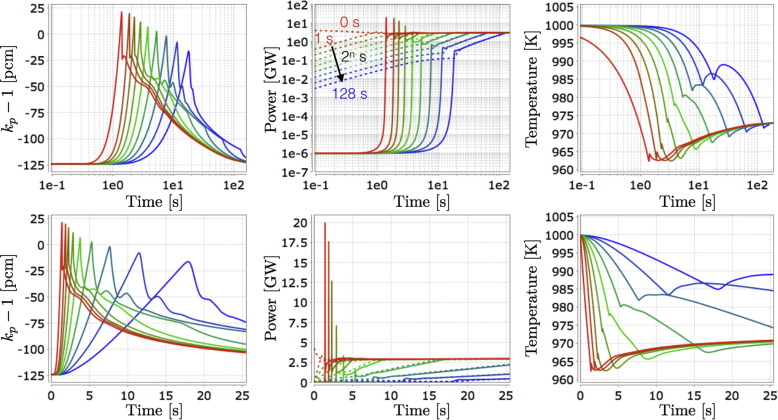
\includegraphics[scale=0.5]{JC-Oct16/overcooling-time.jpg}
                        \end{center}
                        \caption{Evolution of metrics for overcooling of various time constants.}
                        \label{fig:overcool-time}
                \end{figure}
        
        
\end{frame}

\begin{frame}
        \frametitle{Transient Calculations (cont.)}
                Reactivity Insertion:
                \begin{figure}[htbp!]
                        \begin{center}
                        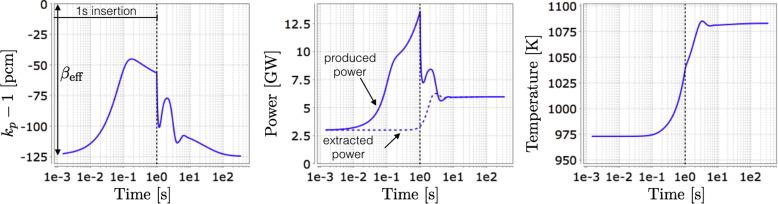
\includegraphics[scale=0.5]{JC-Oct16/ria.jpg}
                        \end{center}
                        \caption{Evolution of metrics for 1000 pcm reactivity insertion in 1 s.}
                        \label{fig:ria}
                \end{figure}
                \begin{figure}[htbp!]
                        \begin{center}
                        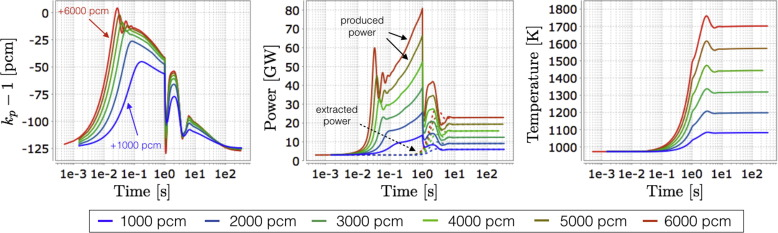
\includegraphics[scale=0.5]{JC-Oct16/ria-variations.jpg}
                        \end{center}
                        \caption{Evolution of metrics for various reactivity insertion in 1 s.}
                        \label{fig:ria-variations}
                \end{figure}
        
        
\end{frame}